\subsection{Components}
To best design the architecture of our system, we must first understand the different actors and their roles. In the FIDO2, OAuth and \acrshort{oidc} specifications there is a degree in ambiguity -- problem being, that while each specification explains details in its own context, the link to other parts of an \acrshort{acs} are not obvious. In this section we identify components of our system and clear this ambiguity by drawing the borders of each specification within the system.

\subsubsection{Requester} 
Requester is the system or application that is requesting access to protected resources on behalf of the user. Typically, this would be an internal or external client application, but it could also be a \acrshort{pacs}.

Client application is the business application the user is about to use. If this is an internal application, it sits within the security perimeter and has direct access to the protected resources. However, it still needs to authenticate the user and verify that the user is authorised to access these resources.

If the client application is is an external application, it typically requires that the user is authenticated and is authorised to use this application. Furthermore, it may require access to user's own resources on their behalf (e.g. user's files) and access to enterprise-owned resources on it's own behalf (e.g. list of departments).
    
The client application can be either of the three client types that are recognised by the OAuth specification~\cite{Hardt2012TheFramework} -- web-based application (running on a web server), user-agent-based application (downloaded from the web server, but executed locally) or a native application. Examples of client application are: Slack, Salesforce, ServiceNow or Zendesk.

The \acrshort{pacs} can also be a requester. Similarly as an internal application, it sits within the security perimeter. It needs to authenticate the users and evaluate whether the user is authorised to pass beyond a certain point in a facility.

\subsubsection{User agent}
User agent does not act on its own, but instead hosts web-based and user-agent based applications. It interacts with the user during login and authentication by displaying login forms communicating with the physical authenticator device via CTAP2 protocol\footnotemark. It is typically a web browser. Principally, it could be both desktop- and mobile-based (currently only on the Android mobile platform). 
% 
\footnotetext{In the FIDO2 terminology, this would be called the \textit{client} or \textit{client device}.}

Examples are Chrome, Mozilla, Microsoft Edge.

\subsubsection{\acrlong{aaserver}} 
The \acrfull{aaserver} is the core of the proposed access control system. As the name suggest, it handles the authentication and authorisation of the users. It communicates with the user agent, the requester, the User directory and the \acrshort{pdp}.
    
\paragraph{User access request}
The \acrshort{aaserver} authenticates the user, when a requester requires access to protected resources on behalf of the user. This flow is activated by a User access request from the requester. If the requester is a client application, the \acrshort{aaserver} supplies a login form. If the requester is a \acrshort{pacs}, the login form is omitted to increase the speed of the process. The \acrshort{aaserver} then communicates with the requester, the User Directory and, optionally with the Authentication front end until the user has been authenticated.

After authentication, the \acrshort{aaserver} proceeds to verify that the user is authorised to access the requested resource. It supplies the necessary information to the \acrshort{pdp} and receives a response with the policy decision.

If the \acrshort{pdp} issued an `Allow access' decision and an OAuth and/or \acrshort{oidc} flow is required, the \acrshort{aaserver} continues the process with the requester until an access token and/or ID token are issued. If the \acrshort{pdp} issued a `Deny access' decision, the \acrshort{aaserver} informs the application and the user that the access has been denied and does not issue the access token or ID token. 

If the OAuth and \acrshort{oidc} are not required (when the requester is an internal application or a \acrshort{pacs}), the \acrshort{aaserver} simply forwards the policy evaluation decision to the requester.

\paragraph{Client access request}
When a requester requires access to protected resources on its own behalf, the user authentication flow is skipped. Instead, the requester begins the process by sending a Client access request to the \acrshort{aaserver}. The client then authenticates using its own set of credentials, using the client credential grant type, as defined by~\cite{Hardt2012TheFramework}. 

The \acrshort{aaserver} verifies the access policy for the requester and if the requester is authorised to access the protected resources, it issues an access token.

The client access request can only be sent by a web-based client (which runs on a server), since native and user-agent-based clients cannot guarantee the security of the client credentials.

\bigskip \noindent
Example of a similar system is Azure AD, discussed in Section~\ref{sec:online-access-control} or ForgeRock Identity Platform\footnotemark.
% 
\footnotetext{\url{https://www.forgerock.com/resources/view/63280622/product-brief/forgerock-identity-platform.pdf}, accessed 10 April 2019.}
    
\subsubsection{Authentication front end}
The Authentication front end is used during user authentication, when the user selects to authenticate using FIDO2 on a smartphone. The Authentication front end is a middle layer between the \acrshort{aaserver} and the smartphone OS, which handles the CTAP2 protocol, and moderates the communication between these two parties.

It receives Authentication Assertions (as defined by~\cite{Balfanz2019Web1}) from the \acrshort{aaserver} and presents these to the smartphone OS, which handles the signing process. Once signed, the Authentication front end returns the assertions to the \acrshort{aaserver}.

The Authentication front end could be a native application, running directly on the smartphone OS, but could also be a browser-based application, if the browser is capable of relying the Authentication assertions to the OS\footnotemark.
% 
\footnotetext{For example Chrome on Android supports the use of WebAuthn and CTAP2~\cite{ChromePlatformStatus2018SupportAPI}.}

\subsubsection{User directory}
% TODO check consistent use accross report
The user directory is a directory service that stores user attributes and can be accessed by the internal systems. The proposed access control system uses the user directory to query attributes about users for authentication and policy evaluation purposes. It also serves attributes to the UserInfo endpoint, when queried.

In addition to standard user attributes (such as name, email, office phone, job title etc.), the user directory stores details about user's authenticators -- the \texttt{credentialPublicKey}(as defined by~\cite{Balfanz2019Web1}) (authenticator's public key). This entry is created when the authenticator is first registered and is used to verify whether the credential challenge for a particular user was signed by an authenticator belonging to this user. Further authenticator details stored in the directory could be the signature counter or a user-defined authenticator name.

The user directory interacts with the \acrshort{aaserver} when it supplies authenticator challenges and verifies authenticator challenge responses. It further interacts with the \acrshort{pdp} where it supplies user attributes, if these are required by the \acrshort{pdp} to evaluate the policy.

Examples of a user directory would be Active Directory\footnote{Active Directory by Microsoft is a subset of Azure AD described in Section~\ref{sec:online-access-control} on page~\pageref{sec:online-access-control}.} or the Apache Directory\footnotemark.
% 
\footnotetext{\url{https://web.archive.org/web/20190407171447/https://directory.apache.org/}, accessed 07 April 2019.}
    
\subsubsection{\acrlong{pdp}}
The \acrfull{pdp} determines whether a given user or requester us authorised to access a protected resource. The \acrshort{pdp} stores the policies and when queried by the \acrshort{aaserver} it evaluates the relevant policy and issues an evaluation decision.

It evaluates the policy based on user/requester attributes, and optionally, additional context information. Some of these attributes are supplied by the \acrshort{aaserver} in the query. If these attributes are not sufficient to evaluate a policy, the \acrshort{pdp} can request additional information from the user directory or the \acrshort{aaserver}.

As specified by requirement
% TODO reference to the correct requirement
, \acrshort{xacml} is used to evaluate access policies. The \acrshort{pdp}, described by the \acrshort{xacml} specification (\cite{OASISStandard2013EXtensible3.0}), cannot operate on its own. Instead it communicates with other components to enforce the policy on the requester. The mapping of the proposed system components to the \acrshort{xacml} context is illustrated in Figure~\ref{fig:xacml-use}, Appendix~\ref{sec:xacml-use} on page~\pageref{fig:xacml-use}.

Example of a solution that implements \acrshort{pdp} functionality is \href{sec:online-access-control}{Azure AD} or WSO2 Identity Server\footnotemark.
% 
\footnotetext{\url{https://web.archive.org/web/20190407180021/https://docs.wso2.com/display/IS570/WSO2+Identity+Server+Documentation}, accessed 07 April 2019.}
    
\subsubsection{Resource Endpoint}
The resource endpoint serves the external clients. This endpoint is the gateway for the external application to access the protected enterprise resources. These resources are divided into scopes the client must present a valid access token for the scope it is attempting to access. The endpoint must verify the validity of the presented token, before it serves the resource. The scopes are defined as \acrshort{api}S, specifying the form of the request and response messages.
    
\subsubsection{UserInfo Endpoint}
The UserInfo endpoint is a component as defined in~\cite{Sakimura2014Final:1}. It serves claims about user attributes to the external clients. The client must present a valid access token to receive the attributes of the associated user. The UserInfo Endpoint serves as an access point for clients outside the security perimeter, but it does not store any user attributes itself. Instead, it queries the User Directory for any requested attributes every time such request is received.

\bigskip\noindent
Not all of the mentioned components are necessarily different physical entities, but we list them here separately as they perform a different function are logically independent. Figure~\ref{fig:data-flow-diagram} presents the high-level view of these components and their interactions. In the next section we describe the interactions between these components in more detail.

\begin{figure}[ht]
    \centering
    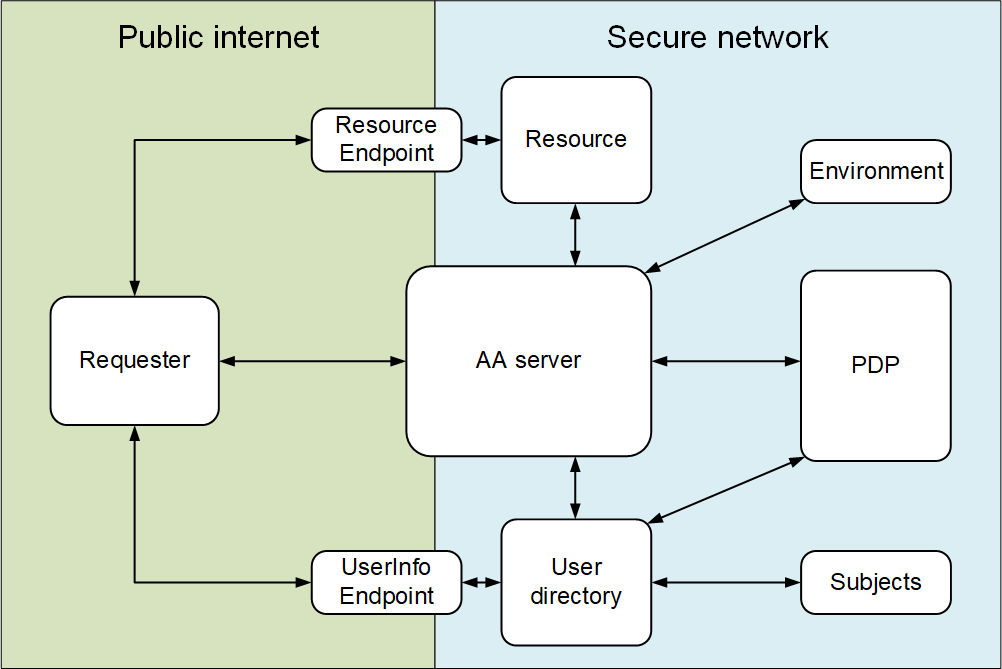
\includegraphics[width=.95\textwidth]{data-flow-diagram}
    \caption{High-level overview of system components and their interactions. The left side of the figure represents unsecured, public internet. The right side represents the security perimeter of the enterprise, which is not accessible from the public internet.}
    \label{fig:data-flow-diagram}
\end{figure}